\documentclass[a4paper,12pt]{article}
\usepackage[utf8]{inputenc}
\usepackage[T1]{fontenc}
\usepackage[french]{babel}
\usepackage{graphicx}
\usepackage{hyperref}
\usepackage{geometry}
\geometry{margin=2.5cm}
\usepackage{setspace}
\onehalfspacing
\usepackage{graphicx}
\usepackage{float}

\begin{document}

% Page de garde
\begin{titlepage}
    \centering
    {\Large \textbf{Université Paris Nanterre}}\\[0.5cm]
    {\large Licence MIASHS - Parcours MIAGE}\\[0.2cm]
    {\large Semestre 4}\\[2cm]

    {\huge \textbf{Rapport de Projet}}\\[0.5cm]
    {\LARGE \textbf{Application de Planification de Voyages}}\\[0.5cm]
    {\LARGE \textit{"TravelDream"}}\\[2cm]

    \textbf{Réalisé par :}\\
    Melissa AKLI \\
    Nikola [Nom de famille] \\[0.5cm]

    \textbf{Encadré par :}\\
    Thibault Anani \\[2cm]

    \vfill
    \textbf{Année universitaire 2024-2025}
\end{titlepage}

\newpage
\tableofcontents
\newpage

\section{Introduction}

\subsection{Contexte du projet}
Dans le cadre du projet S4 de la licence MIASHS parcours MIAGE, nous avons développé l’application web \textit{"TravelDream"} pour aider les utilisateurs à planifier leurs voyages de manière organisée.

\subsection{Objectifs et problématique}
Objectif : créer une plateforme interactive pour :
\begin{itemize}
    \item Gérer les voyages (dates, destinations)
    \item Organiser transports, hébergements, activités
    \item Suivre les dépenses
    \item Consulter une carte interactive
    \item Obtenir des recommandations via un assistant virtuel
\end{itemize}

Problématique : \textbf{Comment simplifier et centraliser la planification de voyages grâce à une interface intuitive et des fonctionnalités complètes ?}

\section{Analyse des Besoins}

\subsection{Besoins fonctionnels}
\begin{itemize}
    \item \textbf{Utilisateurs} : compte, connexion, mot de passe
    \item \textbf{Voyages} : créer, modifier, supprimer, rechercher
    \item \textbf{Activités} : ajouter, planifier, tickets
    \item \textbf{Transports} : type, horaires, détails
    \item \textbf{Logements} : infos, réservations
    \item \textbf{Dépenses} : enregistrement, suivi
    \item \textbf{Extras} : carte interactive, assistant, checklist, restaurants
\end{itemize}

\subsection{Besoins non fonctionnels}
\begin{itemize}
    \item \textbf{Sécurité} : données, mot de passe, injections SQL
    \item \textbf{Utilisabilité} : responsive, rapide, feedback
    \item \textbf{Performance} : requêtes optimisées, multi-utilisateurs
    \item \textbf{Maintenabilité} : MVC, code modulaire
    \item \textbf{Fiabilité} : gestion erreurs, validation, persistance
\end{itemize}

\subsection{Cas d'utilisation}
\begin{itemize}
    \item Créer / gérer un voyage
    \item Planifier les transports
    \item Réserver un hébergement
    \item Organiser les activités
    \item Suivre les dépenses
    \item Utiliser la carte et l’assistant
\end{itemize}

\subsection{Contraintes techniques}
\begin{itemize}
    \item \textbf{Technos} : PHP, MySQL, HTML/CSS/JS, Bootstrap
    \item \textbf{Infra} : serveur local (WAMP/MAMP)
    \item \textbf{Compatibilité} : navigateurs, écrans
    \item \textbf{Intégration} : API Leaflet.js, Nominatim
\end{itemize}
\section{Conception de la Base de Données}
\section{Architecture Technique}

\subsection{Technologies utilisées}
Notre application de planification de voyages \textbf{TravelDream} a été développée à l’aide de technologies modernes et complémentaires :

\paragraph{Backend}
\begin{itemize}
    \item \textbf{PHP 7.4} : Langage côté serveur pour la logique métier, les sessions et la base de données.
    \item \textbf{MySQL 8.0} : SGBD relationnel pour stocker et gérer les données.
    \item \textbf{PDO} : Extension PHP pour accéder à la base de manière sécurisée (requêtes préparées).
\end{itemize}

\paragraph{Frontend}
\begin{itemize}
    \item \textbf{HTML5} : Structure des pages web.
    \item \textbf{CSS3} : Style et présentation visuelle.
    \item \textbf{JavaScript} : Fonctionnalités interactives.
    \item \textbf{Bootstrap 5.3} : Design responsive.
    \item \textbf{Font Awesome 6.4} : Icônes vectorielles.
\end{itemize}

\paragraph{APIs et bibliothèques externes}
\begin{itemize}
    \item \textbf{Leaflet.js} : Carte interactive.
    \item \textbf{Nominatim API} : Recherche de lieux.
    \item \textbf{OpenStreetMap} : Fond de carte.
\end{itemize}

\subsection{Structure du code}

L'application adopte une architecture proche du modèle \textbf{MVC} (non strict).

\paragraph{Organisation générale}
\begin{itemize}
    \item \textbf{Modèle} : Gestion base de données via \texttt{config.php}.
    \item \textbf{Vue} : Fichiers PHP + HTML, stylisés avec CSS.
    \item \textbf{Contrôleur} : Logique dans les fichiers PHP principaux.
\end{itemize}

\paragraph{Sessions}
Sessions initialisées dans \texttt{header.php} via \texttt{session\_start()}, avec vérification via \texttt{isUserLoggedIn()}.

\paragraph{Templates}
Utilisation de templates réutilisables :
\begin{itemize}
    \item \texttt{header.php} : En-tête HTML, barres de navigation, liens CSS.
    \item \texttt{footer.php} : Pied de page, scripts JS.
\end{itemize}

\subsection{Organisation des fichiers}

\paragraph{Fichiers PHP principaux}
\begin{itemize}
    \item \texttt{config.php}, \texttt{header.php}, \texttt{footer.php}
    \item \texttt{inscription.php}, \texttt{pageconnexion.php}, \texttt{Réinitialisation.php}, \texttt{logout.php}
    \item \texttt{destination.php}, \texttt{mesvoyages.php}, \texttt{map.php}, \texttt{chat.php}
\end{itemize}

\paragraph{Fichiers CSS}
\begin{itemize}
    \item \texttt{global.css}, \texttt{style.css}, \texttt{accueil.css}, \texttt{destinations.css}
    \item \texttt{profil\_new.css}, \texttt{chatbot.css}, \texttt{map.css}
\end{itemize}

\paragraph{Ressources statiques}
Stockées dans le dossier \texttt{static} (images, icônes, etc.).

\subsection{Configuration du système}
Cette approche permet de modifier facilement les paramètres de connexion sans avoir à
modifier chaque fichier qui interagit avec la base de données.
\paragraph{Base de données}
Configuration centralisée dans \texttt{config.php} :
\begin{figure}[H]
    \centering
    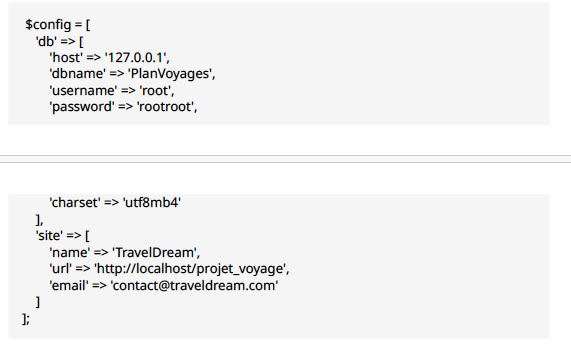
\includegraphics[width=0.8\textwidth]{capture1.png}
    \caption{Capture d’écran de la configuration de la base de données}
\end{figure}


\paragraph{Connexion PDO}
La fonction getDbConnection() dans config.php établit une connexion PDO à la base de données :
\begin{figure}[H]
  \centering
  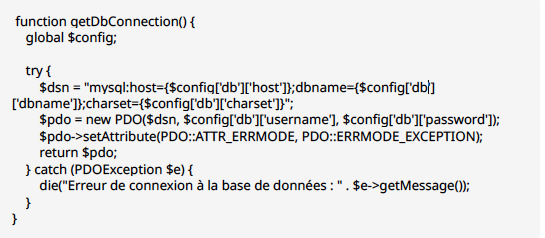
\includegraphics[width=0.95\textwidth]{capture2.png}
  \caption{Fonction PHP de connexion à la base de données}
\end{figure}
Cette fonction configure également PDO pour qu'il lance des exceptions en cas d'erreur,facilitant ainsi le débogage.

\paragraph{Fonctions utilitaires (dans \texttt{config.php})}
\begin{itemize}
    \item \texttt{isUserLoggedIn()} : Vérifie si l’utilisateur est connecté.
    \item \texttt{redirect()} : Redirection vers une page.
    \item \texttt{sanitize()} : Nettoie les données d’entrée.
    \item \texttt{generateAlert()} : Génère des messages Bootstrap.
    \item \texttt{formatDate()} : Formate les dates.
\end{itemize}

\subsection{Sécurité}
\begin{itemize}
    \item Requêtes préparées (PDO) pour éviter les injections SQL.
    \item Mots de passe hachés avec \texttt{password\_hash()}.
    \item Nettoyage des entrées avec \texttt{sanitize()}.
    \item Contrôle d'accès via les sessions.
\end{itemize}

Cette architecture robuste garantit sécurité, maintenabilité et une expérience utilisateur optimale.

\section{Fonctionnalités Implémentées}

\subsection{Module d'Authentification}

Le module d'authentification constitue la porte d'entrée de notre application et assure la sécurité des données utilisateurs.  
Il comprend quatre fonctionnalités principales : l'inscription, la connexion, la réinitialisation du mot de passe et la déconnexion.

\subsubsection{Inscription}

La page d'inscription (\texttt{inscription.php}) permet aux nouveaux utilisateurs de créer un compte sur la plateforme.  
Cette fonctionnalité a été implémentée avec une attention particulière à la sécurité et à l'expérience utilisateur.

\paragraph{Processus d'inscription}

\begin{enumerate}
  \item L'utilisateur accède au formulaire d'inscription via le lien \og S'inscrire \fg{} dans la barre de navigation.
  \item Il remplit les champs requis : nom d'utilisateur, adresse email et mot de passe.
  \item À la soumission, le système vérifie si l'email est déjà utilisé.
  \item Si l'email est disponible, le mot de passe est haché via \texttt{password\_hash()} avant d’être stocké.
  \item Un message de confirmation s’affiche, invitant l’utilisateur à se connecter.
\end{enumerate}

\paragraph{Sécurité}

\begin{itemize}
  \item Utilisation de requêtes préparées pour prévenir les injections SQL.
  \item Hachage du mot de passe avec \texttt{bcrypt} via \texttt{password\_hash()}.
  \item Validation des données côté serveur.
\end{itemize}

\begin{figure}[H]
  \centering
  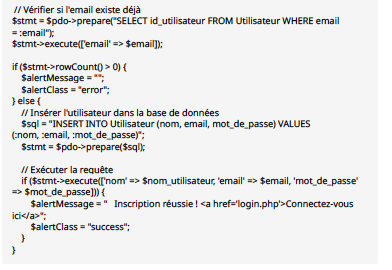
\includegraphics[width=0.9\textwidth]{capture3.png}
  \caption{Interface de la page d'inscription}
\end{figure}
\subsubsection{Connexion}

La page de connexion (\texttt{pageconnexion.php}) permet aux utilisateurs existants d'accéder à leur compte et à leurs données personnelles.

\paragraph{Processus de connexion}

\begin{enumerate}
  \item L'utilisateur accède au formulaire de connexion via le lien \og Connexion \fg{} dans la barre de navigation.
  \item Il saisit son adresse email et son mot de passe.
  \item Le système vérifie l'existence de l'email dans la base de données.
  \item Si l'email existe, le mot de passe est vérifié via \texttt{password\_verify()}.
  \item En cas de succès, les données de l’utilisateur sont stockées en session, puis il est redirigé vers son profil.
  \item En cas d’échec, un message d’erreur est affiché.
\end{enumerate}

\paragraph{Gestion de session}

Après une connexion réussie, les informations suivantes sont stockées en session :
\begin{itemize}
  \item ID de l'utilisateur
  \item Nom d'utilisateur
  \item Adresse email
\end{itemize}

Cela permet d’identifier l’utilisateur et de personnaliser son expérience.

\begin{figure}[H]
  \centering
  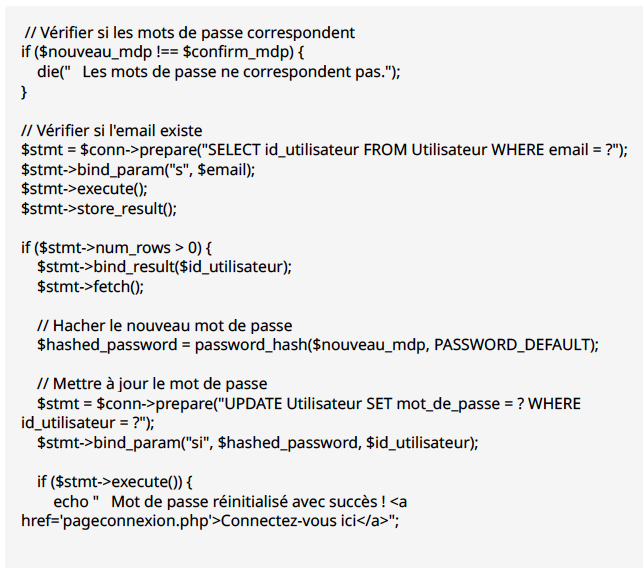
\includegraphics[width=0.9\textwidth]{capture4.png}
  \caption{Interface de la page de connexion}
\end{figure}
\subsubsection{Déconnexion}

\paragraph{Processus de déconnexion}
\begin{enumerate}
  \item L'utilisateur clique sur le lien \og Déconnexion \fg{} dans la barre de navigation.
  \item Le script détruit la session en cours, effaçant toutes les variables de session.
  \item L'utilisateur est redirigé vers la page de connexion.
\end{enumerate}

\paragraph{Sécurité}
\begin{itemize}
  \item Destruction complète de la session pour éviter tout accès non autorisé.
  \item Redirection immédiate pour empêcher toute action après la déconnexion.
\end{itemize}
\begin{figure}[H]
  \centering
  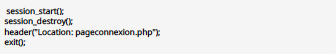
\includegraphics[width=0.9\textwidth]{capture5.png}
  \caption{Interface de la page de connexion}
\end{figure}
\section{Gestion des Voyages}
\subsection{Assistant de voyage (chatbot)}

L'assistant de voyage (\texttt{chat.php}) est un chatbot intelligent qui aide les utilisateurs à trouver des destinations adaptées à leurs préférences.

\paragraph{Fonctionnalités}
\begin{itemize}
  \item Interface de chat intuitive.
  \item Base de données de destinations avec leurs caractéristiques (climat, budget, activités, etc.).
  \item Algorithme de recommandation basé sur les préférences exprimées par l'utilisateur.
  \item Présentation des destinations recommandées avec leurs informations principales.
\end{itemize}

\paragraph{Implémentation technique}
L’assistant est implémenté en JavaScript côté client avec une base de données locale.

\begin{figure}[H]
  \centering
  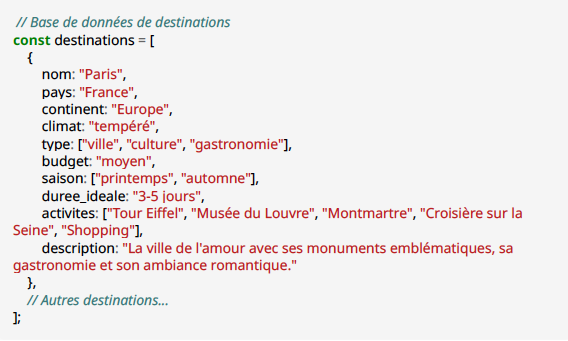
\includegraphics[width=0.9\textwidth]{capture6.png}
\end{figure}
L'algorithme de recommandation filtre les destinations selon les préférences de
l'utilisateur :
\begin{figure}[H]
  \centering
  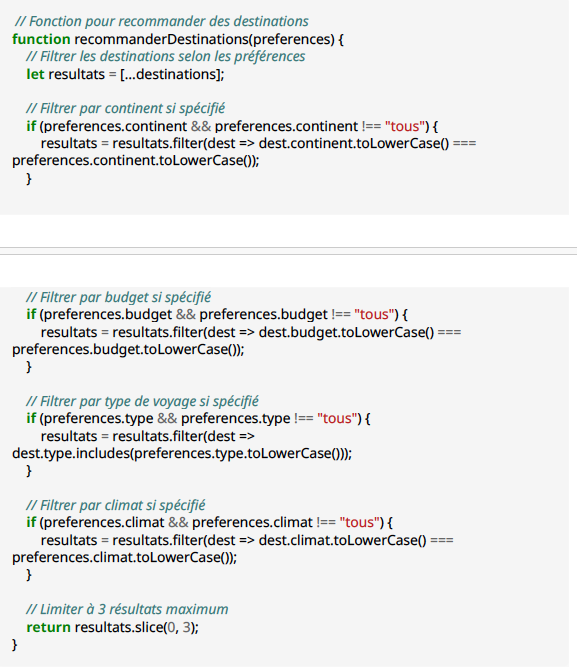
\includegraphics[width=0.9\textwidth]{capture7.png}
\end{figure}
\subsection{Recherche de destinations (destination.php)}

Cette fonctionnalité permet aux utilisateurs de découvrir des lieux de voyage populaires et d’obtenir des informations détaillées sur ceux-ci.

\paragraph{Fonctionnalités}
\begin{itemize}
  \item Affichage des destinations populaires avec images et descriptions.
  \item Barre de recherche pour trouver une destination spécifique.
  \item Affichage détaillé (meilleure période, budget, activités recommandées).
  \item Possibilité de planifier directement un voyage vers la destination choisie.
\end{itemize}

\paragraph{Implémentation technique}
Les informations sont définies dans le code PHP

\begin{figure}[H]
  \centering
  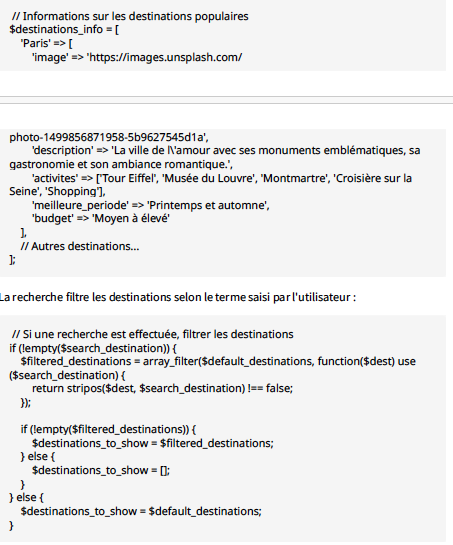
\includegraphics[width=0.9\textwidth]{capture8.png}
\end{figure}
\section{Interface Utilisateur}

\subsection{Charte graphique}
L’interface de l’application \textbf{TravelDream} a été conçue pour offrir une expérience utilisateur agréable, fluide et cohérente. Elle repose sur une charte graphique harmonieuse appliquée à l’ensemble du site.

\subsubsection{Palette de couleurs}
\begin{itemize}
  \item \textbf{Couleur principale} : Bleu ciel (\#4A89DC) – Évoque le ciel, l’océan et la liberté.
  \item \textbf{Couleur secondaire} : Vert tendre (\#48CFAD) – Symbolise la nature et les paysages.
  \item \textbf{Couleur d’accentuation} : Orange (\#FC6E51) – Représente le soleil et l’énergie.
  \item \textbf{Couleurs neutres} : 
  \begin{itemize}
    \item Blanc (\#FFFFFF) – Fond principal pour une lecture confortable.
    \item Gris clair (\#F5F7FA) – Fond secondaire pour distinguer certaines sections.
    \item Gris foncé (\#434A54) – Texte principal pour un bon contraste.
  \end{itemize}
\end{itemize}

\subsubsection{Typographie}
\begin{itemize}
  \item \textbf{Titres} : Montserrat – Moderne, sans-serif, excellente lisibilité.
  \item \textbf{Corps de texte} : Open Sans – Clair et fluide pour le contenu principal.
  \item \textbf{Accents décoratifs} : Pacifico – Cursive utilisée avec parcimonie.
\end{itemize}

\paragraph{Hiérarchie des tailles}
\begin{itemize}
  \item Titres principaux (h1) : 2.5rem
  \item Sous-titres (h2) : 2rem
  \item Titres de section (h3) : 1.5rem
  \item Corps de texte : 1rem
  \item Texte secondaire : 0.875rem
\end{itemize}

\subsubsection{Iconographie}
Nous utilisons la bibliothèque \textbf{Font Awesome} pour des icônes vectorielles adaptables à tous les supports.

\textbf{Utilisations principales :}
\begin{itemize}
  \item Illustration des fonctionnalités (ex : avion, lit)
  \item Navigation (flèches, menu hamburger)
  \item Actions (ajout, modification, suppression)
  \item Statuts (succès, erreur, information)
\end{itemize}

\subsubsection{Éléments d’interface}
\begin{itemize}
  \item \textbf{Boutons} : Coins arrondis, couleur d’action (primaire, secondaire, danger), icône si besoin.
  \item \textbf{Cartes} : Coins arrondis, ombre légère, marges internes.
  \item \textbf{Formulaires} : Champs avec bordures fines, labels clairs, retour visuel de validation.
  \item \textbf{Alertes} : Couleurs distinctes selon le type (succès, erreur, info, avertissement).
\end{itemize}
\subsection{Maquettes et wireframes}

Avant le développement, des maquettes et wireframes ont été réalisés afin de structurer l’interface et garantir une navigation fluide et cohérente.

\subsubsection{Page d'accueil et destinations}

La page d’accueil se compose :

\begin{itemize}
  \item D’un arrière-plan évocateur illustrant l’univers du voyage.
  \item D’un message d’accueil inspirant.
  \item D’une barre de recherche visible et centrale.
  \item D’un affichage en cartes des destinations populaires, chacune avec une image, un nom et un court descriptif.
\end{itemize}

\vspace{0.5cm}
\subsubsection{Pages d'authentification}

Les pages de connexion et d'inscription partagent une structure cohérente :

\begin{itemize}
  \item Un fond d’image représentant le voyage.
  \item Un formulaire centré, épuré et facile à utiliser.
  \item Une interface minimaliste favorisant la concentration de l’utilisateur sur l'action à réaliser.
\end{itemize}

\vspace{0.5cm}

Capture d’écran des pages d’authentification 

\subsubsection{Profil et gestion des voyages}
La page de profil est divisée en deux sections :
\begin{itemize}
  \item À gauche : résumé du profil utilisateur avec statistiques.
  \item À droite : liste des voyages, chaque voyage étant affiché sous forme de carte contenant les informations essentielles et des boutons d'action.
\end{itemize}

\vspace{0.5cm}
\begin{figure}[H]
    \centering
    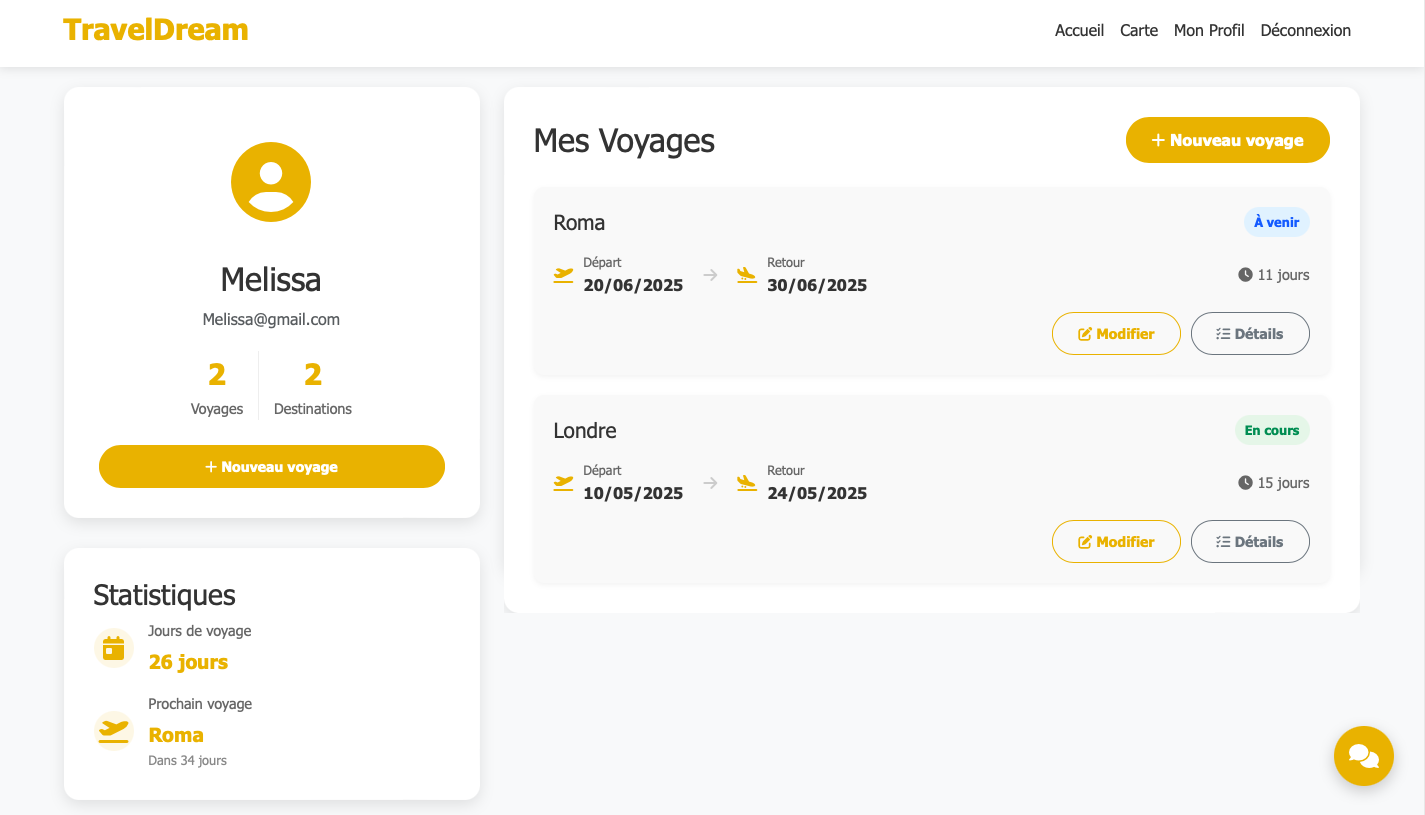
\includegraphics[width=0.85\textwidth]{captures/profil.png}
    \caption{Capture d’écran de la page profil et gestion des voyages.}
\end{figure}

\subsubsection{Carte interactive}
La carte interactive occupe la majeure partie de l’écran et inclut :
\begin{itemize}
  \item Une barre de recherche en haut.
  \item Des boutons de contrôle pour zoom, filtres, etc.
\end{itemize}

\vspace{0.5cm}
\begin{figure}[H]
    \centering
    \includegraphics[width=0.85\textwidth]{captures/carte_interactive.png}
    \caption{Capture d’écran de la carte interactive.}
\end{figure}

\subsubsection{Assistant de voyage (chatbot)}
L’assistant de voyage est présenté en deux colonnes :
\begin{itemize}
  \item À gauche : zone d’informations et de suggestions.
  \item À droite : interface de chat pour l’interaction avec le chatbot.
\end{itemize}

\vspace{0.5cm}
\begin{figure}[H]
    \centering
    \includegraphics[width=0.85\textwidth]{captures/assistant.png}
    \caption{Capture d’écran de l’assistant de voyage.}
\end{figure}

\subsection{Responsive Design}
L’application a été pensée selon une approche \textit{mobile-first} pour assurer une expérience fluide sur tous les types d'appareils.

\subsubsection{Approche technique}
Nous avons utilisé Bootstrap 5 pour garantir une mise en page adaptable :
\begin{itemize}
  \item Système de grille 12 colonnes.
  \item Media queries pour adapter l’affichage.
  \item Classe \texttt{img-fluid} pour rendre les images responsives.
  \item Composants modulables selon la taille d’écran.
\end{itemize}

\subsubsection{Adaptations spécifiques}
Des ajustements ont été appliqués pour améliorer l’expérience utilisateur :
\begin{itemize}
  \item Menu hamburger sur petits écrans.
  \item Cartes de voyage : 3 colonnes (desktop), 2 (tablette), 1 (mobile).
  \item Réorganisation verticale des sections sur mobile.
  \item Champs de formulaire adaptés en largeur.
\end{itemize}
\subsubsection{Tests de compatibilité}
L’interface a été testée sur plusieurs plateformes pour garantir sa compatibilité :
\begin{itemize}
  \item \textbf{Navigateurs} : Chrome, Firefox, Safari, Edge
  \item \textbf{Appareils} : Smartphones (iPhone, Android), tablettes, ordinateurs portables et fixes
  \item \textbf{Tailles d’écran} : de 320px à 1920px de largeur
\end{itemize}

\subsection{Expérience utilisateur}

\subsubsection{Principes d’UX appliqués}
Notre démarche de conception s’est basée sur des principes clés d’UX :
\begin{itemize}
  \item \textbf{Simplicité} : interfaces claires, éléments essentiels uniquement
  \item \textbf{Cohérence} : interactions et design homogènes
  \item \textbf{Feedback} : messages et animations en réponse aux actions utilisateur
  \item \textbf{Accessibilité} : contraste, taille de texte, textes alternatifs pour images
  \item \textbf{Efficacité} : parcours rapides, peu de clics nécessaires
\end{itemize}

\subsubsection{Parcours utilisateur}
Les parcours principaux ont été pensés pour être rapides et intuitifs :
\begin{itemize}
  \item Inscription en 3 étapes maximum
  \item Création de voyage assistée avec validation en temps réel
  \item Recherche de destinations avec suggestions instantanées
  \item Navigation fluide et logique entre les sections
\end{itemize}

\subsubsection{Micro-interactions}
Des micro-interactions ont été intégrées pour renforcer l’engagement :
\begin{itemize}
  \item Animations lors du chargement des cartes
  \item Transitions fluides entre les pages
  \item Effets de survol sur les éléments cliquables
  \item Indicateurs de progression pour les actions longues
\end{itemize}

\vspace{0.5cm}
En résumé, l’interface de \textit{TravelDream} allie esthétique et ergonomie pour une expérience utilisateur agréable et fluide.
\section{Tests et Validation}

\subsection{Stratégie de test}
Pour garantir la qualité et la fiabilité de notre application \textit{TravelDream}, nous avons mis en place une stratégie de test complète couvrant différents aspects du système. Cette approche méthodique nous a permis d'identifier et de corriger les problèmes avant le déploiement final.

\subsubsection{Types de tests implémentés}
Notre stratégie a intégré plusieurs types de tests :
\begin{itemize}
  \item \textbf{Tests unitaires} : vérification du bon fonctionnement de chaque composant (fonctions, classes, modules)
  \item \textbf{Tests d'intégration} : validation des interactions entre les différents modules
  \item \textbf{Tests fonctionnels} : contrôle du respect des exigences pour chaque fonctionnalité
  \item \textbf{Tests d’interface utilisateur} : vérification de l'apparence et du comportement sur divers appareils
  \item \textbf{Tests de sécurité} : identification des vulnérabilités, notamment sur l’authentification et la gestion des données
\end{itemize}

\subsubsection{Environnement de test}
Les tests ont été réalisés dans un environnement dédié, proche de la production :
\begin{itemize}
  \item Serveur local WAMP/MAMP avec configuration équivalente à celle de production
  \item Base de données de test avec des jeux de données réalistes
  \item Navigateurs : Chrome, Firefox, Safari, Edge
  \item Appareils : ordinateurs, tablettes, smartphones
\end{itemize}

\subsubsection{Outils et méthodes}
Nous avons utilisé les outils suivants pour le processus de validation :
\begin{itemize}
  \item \textbf{Tests manuels} : scénarios exécutés manuellement avec documentation des résultats
  \item \textbf{Validation W3C} : conformité HTML/CSS aux standards du web
  \item \textbf{Outils développeur navigateur} : inspection DOM, débogage JavaScript, analyse performance
  \item \textbf{Checklists} : vérification systématique des fonctionnalités via des listes de contrôle
\end{itemize}

\subsection{Tests fonctionnels}
Les tests fonctionnels ont permis de valider que chaque fonctionnalité respecte les besoins utilisateurs et les spécifications définies.
\subsection{Tests d'intégration}
Les tests d'intégration ont permis de vérifier que les différents modules de l'application fonctionnent correctement ensemble.

\subsubsection{Flux complets}
Plusieurs flux d’utilisation ont été testés :
\begin{itemize}
  \item \textbf{Inscription → Connexion → Création d’un voyage → Ajout d’activités → Visualisation} : vérification de l’enregistrement correct des données et de leur liaison.
  \item \textbf{Recherche de destination → Planification d’un voyage → Ajout à la liste personnelle} : vérification de la reprise des données de destination et de l’intégration avec la création de voyage.
  \item \textbf{Utilisation de la carte → Enregistrement d’un lieu → Association à un voyage} : vérification de l’enregistrement des coordonnées et de l’intégration avec la gestion des voyages.
\end{itemize}

\subsubsection{Intégrité des données}
L'intégrité des données a été contrôlée pour :
\begin{itemize}
  \item Création, modification et suppression de voyages et d’activités
  \item Vérification des contraintes d'intégrité référentielle (clés étrangères)
  \item Cohérence des données entre les différentes tables
\end{itemize}
\section{Difficultés Rencontrées et Solutions}

\subsection{Problèmes techniques}
Durant le développement de l’application \textit{TravelDream}, plusieurs défis techniques ont été rencontrés, nécessitant des solutions adaptées.

\subsubsection{Gestion des sessions utilisateurs}
\textbf{Problème} : Déconnexions inattendues et problèmes d’accès aux données de session entre les pages.\\
\textbf{Solution} : Centralisation de la gestion dans \texttt{header.php} avec \texttt{session\_start()} au début. Création de \texttt{isUserLoggedIn()} dans \texttt{config.php} pour une vérification cohérente.

\subsubsection{Compatibilité entre navigateurs}
\textbf{Problème} : Affichage incohérent des éléments d’interface (formulaires, flexbox).\\
\textbf{Solution} : Utilisation de Bootstrap, ajout de préfixes CSS et tests sur Chrome, Firefox, Safari et Edge.

\subsubsection{Performances de la carte interactive}
\textbf{Problème} : Temps de chargement longs et consommation élevée de ressources.\\
\textbf{Solution} : Optimisation de Leaflet.js en :
\begin{itemize}
  \item Limitant le nombre de marqueurs
  \item Utilisant un chargement différé des tuiles
  \item Implémentant un cache des résultats fréquents
  \item Ajoutant un délai entre les requêtes API
\end{itemize}

\subsection{Défis d’implémentation}

\subsubsection{Système de recommandation de l’assistant de voyage}
\textbf{Problème} : Difficulté à générer des suggestions personnalisées pertinentes.\\
\textbf{Solution} : Création d’une base de données structurée (climat, budget, activités) + algorithme de filtrage par critères.

\subsubsection{Gestion des dates et fuseaux horaires}
\textbf{Problème} : Difficultés liées aux fuseaux horaires et au formatage.\\
\textbf{Solution} :
\begin{itemize}
  \item Format SQL (YYYY-MM-DD) pour la base
  \item Fonction \texttt{formatDate()} dans \texttt{config.php}
  \item Utilisation de \texttt{DateTime} de PHP
  \item Stockage explicite du fuseau horaire
\end{itemize}
\subsubsection{Formulaires dynamiques}
\textbf{Problème} : Affichage conditionnel de champs supplémentaires selon les choix utilisateur (ex : tickets).\\
\textbf{Solution} : Utilisation de JavaScript pour modifier dynamiquement les champs, avec validation serveur en complément.

\subsection{Solutions apportées}

\subsubsection{Méthodologie de résolution de problèmes}
Nous avons adopté une démarche structurée :
\begin{enumerate}
  \item Identification précise du problème (comportement observé vs attendu)
  \item Analyse des causes potentielles (code, logs, conditions de reproduction)
  \item Recherche de solutions (documentation, forums, bonnes pratiques)
  \item Implémentation et tests en environnement de développement
  \item Validation de la résolution sans effets de bord
  \item Documentation des solutions pour référence future
\end{enumerate}

\subsubsection{Refactorisation et amélioration continue}
\begin{itemize}
  \item Revues de code régulières
  \item Refactorisation progressive
  \item Standardisation des pratiques (conventions, patterns réutilisables)
  \item Documentation technique à jour
\end{itemize}

\subsubsection{Apprentissages clés}
Ces défis nous ont permis d’acquérir :
\begin{itemize}
  \item L’importance d’une architecture bien pensée dès le départ
  \item La valeur des tests réguliers
  \item La nécessité d’une approche pragmatique
  \item Les bénéfices d’une documentation claire et d’un code commenté
\end{itemize}

La résolution de ces problèmes a renforcé nos compétences et la qualité de l’application.
\section{Améliorations Futures}

\subsection{Fonctionnalités à développer}

\subsubsection{Partage de voyages}
\textbf{Objectif} : Permettre aux utilisateurs de partager leurs voyages.\\
\textbf{Implémentation envisagée} :
\begin{itemize}
  \item Table de partage dans la base de données
  \item Gestion des droits (lecture/modification)
  \item Liens de partage uniques et sécurisés
  \item Interface de gestion des collaborateurs
\end{itemize}

\subsubsection{Application mobile native}
\textbf{Objectif} : Développer des applications natives iOS/Android synchronisées avec la version web.\\
\textbf{Avantages} :
\begin{itemize}
  \item Accès hors ligne
  \item Fonctionnalités natives (GPS, caméra, notifications)
  \item Expérience optimisée
  \item Notifications push
\end{itemize}

\subsubsection{Intégration avec des services externes}
\textbf{Objectif} : Enrichir l'application avec des APIs externes.\\
\textbf{Services ciblés} :
\begin{itemize}
  \item Réservations (Booking, Expedia)
  \item Vols (Skyscanner, Kayak)
  \item Recommandations (TripAdvisor, Google Places)
  \item Météo et convertisseurs de devises
\end{itemize}
\textbf{Bénéfices} : Centralisation, données à jour, richesse fonctionnelle.

\subsubsection{Système de budgétisation avancé}
\textbf{Fonctionnalités envisagées} :
\begin{itemize}
  \item Budget global et par catégorie
  \item Suivi réel vs prévu
  \item Graphiques de dépenses
  \item Support multi-devises avec conversion
\end{itemize}

\subsection{Optimisations techniques}

\subsubsection{Architecture MVC complète}
\textbf{État actuel} : MVC partiel.\\
\textbf{Amélioration proposée} :
\begin{itemize}
  \item Dossiers modèles, vues, contrôleurs
  \item Utilisation d’un moteur de templates
\end{itemize}
\textbf{Bénéfices} : Code plus clair, maintenable, testable.

\subsubsection{API RESTful}
\textbf{Objectif} : Permettre une communication multi-interfaces (web, mobile).\\
\textbf{Implémentation} :
\begin{itemize}
  \item Endpoints REST pour les fonctions principales
  \item Authentification via JWT
  \item Documentation Swagger
  \item Versioning
\end{itemize}

\subsubsection{Amélioration des performances}
\begin{itemize}
  \item \textbf{Cache} : Redis ou Memcached
  \item \textbf{Requêtes SQL} : Indexation, optimisation
  \item \textbf{Lazy loading} : Images et contenus lourds
  \item \textbf{Minification} : CSS/JS
  \item \textbf{CDN} : Ressources statiques
\end{itemize}
\subsubsection{Renforcement de la sécurité}
\textbf{Mesures envisagées} :
\begin{itemize}
  \item Authentification à deux facteurs (2FA)
  \item Audit de sécurité et corrections des vulnérabilités
  \item Chiffrement des données sensibles
  \item Protection CSRF via tokens
  \item Rate limiting contre les attaques par force brute
\end{itemize}

\subsection{Évolutions possibles}

\subsubsection{Fonctionnalités sociales et communautaires}
\textbf{Objectif} : Créer une plateforme sociale pour voyageurs.\\
\textbf{Fonctionnalités potentielles} :
\begin{itemize}
  \item Profils publics
  \item Partage de récits/photos de voyage
  \item Suivi entre utilisateurs
  \item Forums par destination
  \item Avis et notations sur lieux/activités
\end{itemize}

\subsubsection{Intelligence artificielle et personnalisation}
\textbf{Objectif} : Offrir une assistance intelligente via l'IA.\\
\textbf{Applications possibles} :
\begin{itemize}
  \item Recommandations personnalisées
  \item Assistant virtuel (NLP)
  \item Analyse prédictive des meilleures périodes
  \item Itinéraires adaptés aux préférences
\end{itemize}

\subsubsection{Réalité augmentée pour l'exploration}
\textbf{Objectif} : Enrichir l'exploration via la RA.\\
\textbf{Applications possibles} :
\begin{itemize}
  \item Visualisation RA des points d’intérêt
  \item Informations culturelles superposées
  \item Guides virtuels en RA
  \item Traduction en temps réel via caméra
\end{itemize}

\textbf{Conclusion} : Ces évolutions permettraient à \textit{TravelDream} de passer d’un outil de planification à une véritable plateforme immersive et personnalisée dédiée aux voyageurs.
\section{Conclusion}

\subsection{Synthèse du projet}
Le projet \textit{TravelDream} a permis de concevoir une application web complète dédiée à la planification de voyages. Elle centralise toutes les étapes d’organisation : 
\begin{itemize}
  \item Création et gestion de voyages
  \item Organisation des transports et hébergements
  \item Planification d’activités
  \item Gestion du budget
  \item Carte interactive
  \item Recommandations personnalisées
\end{itemize}
L’architecture repose sur PHP, MySQL, JavaScript et Bootstrap. Elle est modulaire, maintenable, et s’appuie sur une base de données bien structurée. L’interface est responsive, intuitive, et les tests ont abouti à un produit stable.

\subsection{Compétences acquises}
\textbf{Compétences techniques} :
\begin{itemize}
  \item Développement web full-stack (frontend/backend)
  \item Conception et implémentation de bases de données relationnelles
  \item Programmation orientée objet en PHP
  \item Sécurité web (protection contre vulnérabilités)
  \item Intégration d’APIs tierces (cartes, services)
  \item Responsive design
  \item Tests et débogage
\end{itemize}

\textbf{Compétences transversales} :
\begin{itemize}
  \item Gestion de projet
  \item Travail en équipe
  \item Résolution de problèmes
  \item Documentation technique
  \item UX/UI design
  \item Veille technologique
\end{itemize}

\subsection{Bilan personnel}
\textbf{Réussites} :
\begin{itemize}
  \item Architecture solide
  \item Interface intuitive et esthétique
  \item Carte interactive et assistant fonctionnels
  \item Résolution de bugs
  \item Bonne collaboration d’équipe
\end{itemize}

\textbf{Difficultés surmontées} :
\begin{itemize}
  \item Gestion des sessions et de l’authentification
  \item Optimisation des performances (carte)
  \item Adaptation multi-appareils
  \item Intégration des modules en équipe
\end{itemize}

\textbf{Enseignements tirés} :
\begin{itemize}
  \item Importance de la conception initiale (base de données)
  \item Tests réguliers
  \item Documentation continue
  \item Prise en compte des retours utilisateurs
  \item Adaptabilité technique
\end{itemize}

\subsection{Perspectives}
\textit{TravelDream} constitue une base solide avec des perspectives d’évolutions majeures :
\begin{itemize}
  \item Application mobile
  \item Fonctionnalités sociales
  \item IA pour recommandations
  \item Réalité augmentée
  \item Analyse de données
  \item Blockchain pour sécurité des réservations
\end{itemize}

Ce projet de S4 en licence MIASHS-MIAGE nous a permis d’appliquer nos acquis, de progresser techniquement et humainement, et de livrer une application aboutie, répondant à des besoins concrets.

\end{document}
